\section{Randomized Algorithms}
\paragraph{Random Algorithm} In the algorithm you compute something random. So on the same input you don't have to get the same output.\\ \\
You can't say, every run gives the optimal solution. But you can get the probability with that you get the optimal solution. \\
\begin{center}
\begin{tabular}{|c|c|c|c|}\hline
	opt. Result & exact Alg & rand Alg (2)& Approx (1)\\ \hline 
	100 & 100 & 100 & 92\\
	100 & 100 & 8& 93\\
	100 & 100 & 90& 99 \\
	100 & 100 & 99& 100 \\
	100 & 100 & 100 & 91\\
	100 & 100 & 100 & 92\\\hline 
\end{tabular}
\end{center}
(1) know that the approximation is very close \\
(2) expect to be very close in p of cases \\


\subsection{Example}
Two Polynomials:
$$P(x) = (x+1)(x-2)(x+3)(x-4)(x+5)(x-6)$$
$$Q(x) = x^6 - 7x^3 + 25$$
$$P(x) \stackrel{?}{\equiv} Q(x)$$
Check $x=2$ ($P$ will evaluate to 0), but
$$Q(2) = 2^6 - 7 \cdot 2^3 + 25 = 33 \neq 0$$
So we can say $P(x) \not \equiv Q(x)$ with $P=1$. \\ If selected number right $\Rightarrow$ $P(x) \not \equiv Q(x)$ with $P < 1$. \\
The random part is to choose $x=2$.  
$$P(x) = x^2 + 7x +1$$
$$Q(x) = (x+2)^2$$
$$P(1) = 1 + 7 + 1 = 9  = (1+2)^2 = Q(1)$$
Choose $x$ from a range of numbers (1...100). \\
Good numbers: $P(x)$ and $Q(x)$ evaluate to different results. \\
Bad numbers: They evaluate to the same result. \\
So how many bad numbers do we have? 
$$F(X) = P(X) - Q(X)$$
If they are equivalent $F$ would evaluate to 0 all the time. The bad numbers are those with $F =$ 0 ($F(3) = P(3) - Q(3) = 0$). Number of bad numbers $\leq d$ where $d$ is the degree of the polynomial. Get a very large range ($d \cdot 100$)so you have many good numbers. So the probability for a bad number is
$$P_{bad} = \frac{d}{100 \cdot d} = \frac{1}{100}$$
One would differentiate between the following two types of randomized algorithms
\begin{itemize}
	\item Monte Carlo: takes polynomial time, gets the right/optimal solution with expected probability
	\item Las Vegas: sure that the right/optimal solution will be found, takes expected polynomial time
\end{itemize}
$$\text{Monte-Carlo} \stackrel{\text{repeat } \infty \text{-many times}}{\rightarrow} \text{Las Vegas}$$
Example from last time: \\
If $\exists x^* P(x^*) \neq Q(x^*) \Rightarrow P(x) \not \equiv Q(x)$\\
$P(x) = x^3 + 2 x^2 - 3x, Q(x) = (x-1)(x^2+2) = x^3+2x-x^2-2$ \\
$P(1) = 0 = Q(1) \Rightarrow $ don't know  whether $P(x) \equiv Q(x)$ \\
$P(2) = 10 \neq 6 = Q(2) \Rightarrow P(x) \not \equiv Q(x) $ \\
Correct answer with some probability. \\
Extract number out of a certain range $[0,100]$. How many good numbers (evaluate to different solutions) and bad (to the same result) are there? \\
Look at: $F(x) = P(x) - Q(x)$ \\
$F(x) = 0 \Leftrightarrow P(x) \equiv Q(x)$ \\
Roots of $F(x)$: "bad numbers" only a few where $F(x) = 0$ \\
\paragraph{Question:} how many "bad numbers" are there? \\
$\Rightarrow$ suppose $deg(Q) = deg(P) = d \Rightarrow d $ bad numbers at most ($\leq d$) \\
Instead of fixed range choose $[0,100 \cdot d]$ \\
$\Rightarrow$ good numbers are $1 - \frac{d}{100d} = 99\%$\\
$\Rightarrow $ increase the range proportionally to $d$ (Monte-Carlo-Algorithm) \\
To increase the probability \\
\begin{itemize}
	\item increase range
	\item repeat the algorithm several times
\end{itemize}
Probability after 2 or $k$ solutions respectively 
$$\frac{1}{100} \cdot \frac{1}{100} = \frac{1}{100^2} \Rightarrow \frac{1	}{100^k}$$
$1-\frac{1}{100^k}$ can make solution arbitrarily close to 1. \\
Also a correct answer is given in one of cases with probability 1 - the "no"-answer. \\
repetition-probabilities for bad numbers
$$\underbrace{\frac{d}{100d} \cdot \frac{d-1}{100d-1} \cdot \frac{d-2}{100d-1}}_{\stackrel{\rightarrow}{\text{prob. gets better/prob. decreases(}\Rightarrow\text{no independent repetitions)}}}$$
if $k>d \Rightarrow \frac{0}{100d-k}$ \\
if $K=d+1$ repetitions the correct solution is found but $\mathcal{O}(d) \cdot d+1 = \mathcal{O}(d^2)$ \\
\paragraph{Complexity} $\mathcal{O}(d\cdot k)$ ($d \rightarrow$ per step, $k \rightarrow$ number of repetitions). \\
Good is $k<<d \Rightarrow$ Complexity stays $\mathcal{O}(d)$ randomization is done to get an efficient algorithm. 
\paragraph{More general formulation} 
conditional probability \\
two events: $w_1,w_2$ \\
independence: $w_1 \Rightarrow Pr(w_1), w_2 \Rightarrow Pr(w_2)$ \\
non-independence: $w_1 \Rightarrow Pr(w_1), w_2 \Rightarrow Pr(w_1|w_2)$ \\
if independence is given $\Rightarrow Pr(w_2) = Pr(w_2|w_1)$ \\
if dependence is given $\Rightarrow Pr(w_2|w_1) = \frac{Pr(w_2 \cap w_1)}{Pr(w_1)}$ \\
events $w_1,w_2$: 
\begin{align*}
P(w_2|w_1) &= \frac{P(w_2 \cap w_1)}{P(w_1)} \\
P(w_1 \cap w_2) &= P(w_2|w_1) \cdot P(w_1) \\
P(w_1 \cap w_2) &= P(w_2) \cdot P(w_1) & | \text{if independent}
\end{align*}
let $w_i := $ get bad numbers at step/repetition $i$
$$P(w_1 \cap w_2 \cap ... \cap w_k) = ?$$ 
correct $W' = 1 -P(w_1 \cap w_2 \cap ... \cap w_k)$
\begin{align*}
	P(w_1 \cap w_2 \cap ... \cap w_k) &= P(w_k|w_{k-1} \cap ... \cap w_1) \cdot P(w_1 \cap ... \cap w_{k-1}) \\
	&= P(w_k|w_{k-1} \cap ... \cap w_1) P(w_{k-1}|w_{k-1} \cap ... \cap w_1) \cdot P(w_1 \cap ... \cap w_{k-2}) \\
	&= \left( \prod_{i=2}^{k} \left(P|w_1 \cap ... \cap w_{i-1} \right) \right) \cdot P(w_1)
\end{align*}
\subsection{Random Walk}
Search space \includegraphics[scale=0.2]{randomizedAlg/opt-way.jpg} optimal Solution \\
do from every point a random choice and walk down the chosen path \\
$-n-...-\stackrel{you}{\underbrace{0}_{0.5 \leftarrow \rightarrow 0.5}}------------------\stackrel{\times}{n}$ \\
Probability of doing a step with $\frac{1}{p}$ and $1-\frac{1}{p}$ in the other direction. Want to estimate $\# steps$ to reach $n$. $w: $ event $you$ reaches $\times$, $Pr(w)=?$ \\
$Z:$ random variable = $\# steps$ before reaching $\times$ \\
Try to compute the expected value 
\begin{align*}
	E[Z] &= ? \\
	E[Z] &= \sum_i(i \cdot P(Z=i)) & |i \in \{\text{values $Z$ can take}\}
\end{align*}
\paragraph{Example} dice \\
$Z = $ numbers on dice 
\begin{align*}
E(Z) &= \frac{1}{6} \cdot 1 + \frac{1}{6} \cdot 2 + \frac{1}{6} \cdot 3 + \frac{1}{6} \cdot  4 + \frac{1}{6} \cdot 5 + \frac{1}{6} \cdot 6 \\
&= 1 \cdot P(Z=1) + 2 \cdot P(Z=2) + ... + 6 \cdot P(Z=6) \\
&= 3.5
\end{align*}

\subsubsection{Random Walker} $0--------(i-1)\stackrel{\leftarrow}{-}\stackrel{\mathwitch}{i}\stackrel{\rightarrow}{-}(i+1)---------n-\rightarrow $ \\
$Pr(i \rightarrow i+1) = \frac{1}{2}$, $Pr(i \rightarrow i-1) = \frac{1}{2}$ \\
Initially $\mathwitch$ is at position 0. $\rightarrow$ What is the expected number of steps that $\mathwitch$ needs to reach $n$? \\
$X_i$ the random variable that corresponds to the number of moves that $\mathwitch$ needs to reach $i$. Find $E[X_n]$. Sei $T(i) = E(X_i)$ \\
\begin{align*}
	t(0) &= 0 \\
	t(1) &= 1 + \frac{1}{2} \cdot t(0) + \frac{1}{2} \cdot t(2) \\
	&... \\
	t(i) &= 1 + \frac{1}{2} \cdot t(i-1) + \frac{1}{2} \cdot t(i+1) \\
	&... \\
	t(n-1) &= 1 + \frac{1}{2} \cdot t(n-2) + \frac{1}{2} \cdot t(n) \\
	t(n) &= 1 + \frac{1}{2} \cdot t(n-1) & |unique
\end{align*}
\begin{center}
    $\left.\begin{aligned}
t(n-1) = 1 + \frac{1}{2} \cdot t(n-2) + \frac{1}{2} (1 + \cdot t(n-1)) \\
\Leftrightarrow \frac{1}{2} t(n-1) = \frac{3}{2} +  \frac{1}{2}t(n-2) \\
\Leftrightarrow t(n-1) = 3 + t(n-2) \\ \phantom{t} \\ 
t(n-2) = 1+\frac{1}{2}t(n-3) + \frac{1}{2} (3+t(n-2)) \\
\Leftrightarrow \frac{1}{2}t(n-2) = \frac{5}{2} + \frac{1}{2} t(n-3) \\
\Leftrightarrow t(n-2) = 5 + t(n-3) \\ ... \\
t(n-i) = 1 + 2i + t(n-i-1) \\
t(1) = 1 + 2 (n-1) + t(0) = 1 + 2(n-1)
\end{aligned}\right\rbrace$Backward-Propagation
\end{center}
\begin{center}
	$\left.\begin{aligned}
	t(1) = 1 + 2(n-1) \\
	t(2) = 1 + 2(n-1) + 1 + 2(n-1)  \\ = 3 + 2((n-1)+(n-2)) \\
	... \\
	t(n) = n + 2((n-1)+(n-2)+...+0) \\
	= n+2 \frac{(n-1)n}{2}  \\= n + n^2 - n = n^2
	\end{aligned}\right\rbrace$Forward-Propagation
\end{center}

\subsubsection{2-SAT}
\paragraph{Input} A logical formula $\Phi$ with $n$ variables and $m$ clauses each with 2 literals
\paragraph{Example} $\Phi = (x_1 \lor \overline{x_2}) \land (\overline{x_2} \lor \overline{x_3}) \land (x_1 \lor x_2) \land (\overline{x_1} \lor \overline{x_4})$
\paragraph{Output} An assignment of the truth values of each variable of $\Phi$ that make $\Phi$ satisfiable.
\paragraph{Example} $x_1=true;x_3=false;x_4=false,x_2=true$
\paragraph{A randomized algorithm} 
\begin{verbatim}
Start with arbitrary assignment (e.g. xi = false forall i=1,...,n) 
while(exists an unsatisfied clause ) [or tired flipping coins]
  c <- some unsatisfied clause
  choose a variable of c by flipping a coind
  change the value of the variable
\end{verbatim}
\paragraph{Example} $x_1=x_2=x_3=x_4=false$ \\
$(x_1 \lor x_2)$ chosen $\rightarrow x_2=true$ \\
$(x_1 \lor \overline{x_2})$ chosen $\rightarrow x_2=false$ \\
... \\
$\mathwitch -----------------------------S-----\rightarrow$ \\
What is $Pr \rightarrow ?$, What is $Pr \leftarrow ?$ \\
$S \leftarrow$ a (any) truth assignment of $\Phi$ \\
$A_j \leftarrow$ the assignment of values to the variables of $\Phi$ after the $j$-th iteration \\
$X_i \leftarrow$ the number of variables that have the same value in $A_j$ and $S$. \\
If $X_j = n \Rightarrow S=A_j$ \\
$\left.\begin{aligned}
S = x_1 = t, x_3=t,x_4=f, x_2 = t \\
A_0=x_1=x_2=x_3=x_4=f
\end{aligned}\right\rbrace X_0=2$ 
$x_0:$ How many do the two sets have in common ($X_j=(A_j\cap S)$) 
\paragraph{Claim} If $\Phi$ has a truth assignment $S$ making it true, then in $n^2$ iterations the algorithm is expected to find $S$.
\subparagraph{Proof}$\mathwitch --------------------------S(X_j=n)-----\rightarrow$ \\
Wlog ("without loss of generality") $X_0 = 0$ \\
What is the probability that at some iteration $j$ $\mathwitch$ moves closer/further away from $S$? \\
$Pr(X_{j+1} = k+1|X_{j=k}) \rightarrow \mathwitch$ moves closer \\ 
$Pr(X_{j+1} = k-1|X_{j=k}) \rightarrow \mathwitch$ moves away \\
$(x_k,x_{\lambda}) \rightarrow $ the unsatisfied clause of the $j$-th iteration \\
$\rightarrow$ \textit{Observation: $(x_k,x_{\lambda})$ cannot have the same value as $S$. At least one of the $x_k,x_{\lambda}$ must have a different value in $S_i$, otherwise $(x_k,x_{\lambda})$ satisfied}
\begin{itemize}
	\item Both have different values: $P(closer) = 1$
	\item Exactly one has a different value: $P(closer) = \frac{1}{2} = P(away)$
\end{itemize}
\paragraph{Theorem} If the algorithm makes $sn^2$ iterations and $S$ is satisfiable, then $Pr(\text{not finding }S) \leq \frac{1}{2}$
\subparagraph{Proof} $X \leftarrow$ random variable that corresponds to the number of iterations to find $S \stackrel{\text{Random\\Walker}}{\Rightarrow} E(X) = n^2$ \\
$Pr(\text{not finding S}) = Pr(X > 2n^2) \stackrel{Markov Inequality}{\leq} \frac{E[X]}{2n^2} ) = \frac{1}{2}$ 
\paragraph{Markov Inequality} $Pr(X \geq \alpha) \leq \frac{E(X)}{\alpha}$
\subparagraph{Proof} 
\begin{align*}
	E(X) &= \sum_{i=0}^{\infty}Pr(X=i) \\
	&= \underbrace{\sum_{i\geq\alpha} iPr(X=i)}_{\geq 0} + \underbrace{\sum_{i<\alpha}iPr(X=i)}_{\geq 0} \\
	&\Rightarrow E(X) \geq \sum_{i \geq \alpha}iPr(X=i) \geq \alpha \sum_{I \geq \alpha}Pr(X=i)
\end{align*}
\paragraph{2-SAT is in P} $\Phi = (\overline{x} \lor y) \land (\overline{\text{\textcolor{orange}{$y$}}} \lor \text{\textcolor{orange}{$z$}}) \land (\text{\textcolor{red}{$z$}} \lor \text{\textcolor{red}{$y$}})$ \\
$x \lor y \Leftrightarrow \overline{x} \Rightarrow y \Leftrightarrow \overline{y} \Rightarrow x$ \\
Based $\Phi$ creates a graph $G_{\Phi}$: $\forall$ variable $x \in \Phi$, $G_{\phi}$ has two vertices $x, \overline{x}$ \\
example $G_{\Phi}:$ \\
\begin{center}
	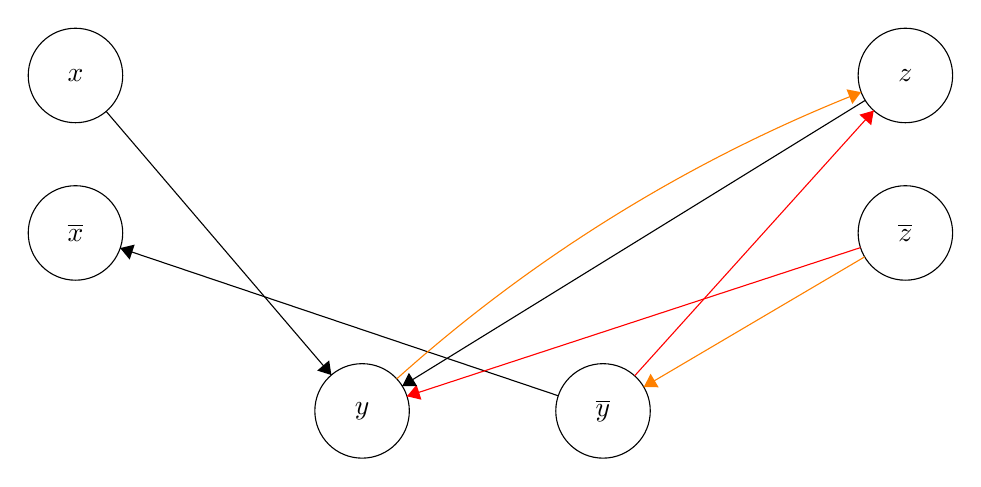
\begin{tikzpicture}[scale=0.2]
	\tikzstyle{every node}+=[inner sep=0pt]
	\draw [black] (9.3,-24.7) circle (3);
	\draw (9.3,-24.7) node {$x$};
	\draw [black] (9.3,-34.7) circle (3);
	\draw (9.3,-34.7) node {$\overline{x}$};
	\draw [black] (27.5,-46) circle (3);
	\draw (27.5,-46) node {$y$};
	\draw [black] (42.8,-46) circle (3);
	\draw (42.8,-46) node {$\overline{y}$};
	\draw [black] (62,-24.7) circle (3);
	\draw (62,-24.7) node {$z$};
	\draw [black] (62,-34.7) circle (3);
	\draw (62,-34.7) node {$\overline{z}$};
	\draw [black] (11.25,-26.98) -- (25.55,-43.72);
	\fill [black] (25.55,-43.72) -- (25.41,-42.79) -- (24.65,-43.44);
	\draw [black] (39.96,-45.04) -- (12.14,-35.66);
	\fill [black] (12.14,-35.66) -- (12.74,-36.39) -- (13.06,-35.44);
	\draw [orange] (59.41,-36.22) -- (45.39,-44.48);
	\fill [orange] (45.39,-44.48) -- (46.33,-44.5) -- (45.82,-43.64);
	\draw [orange] (29.702,-43.963) arc (131.89631:111.48533:97.804);
	\fill [orange] (59.19,-25.76) -- (58.26,-25.58) -- (58.63,-26.51);
	\draw [red] (59.15,-35.63) -- (30.35,-45.07);
	\fill [red] (30.35,-45.07) -- (31.27,-45.29) -- (30.96,-44.34);
	\draw [black] (59.45,-26.28) -- (30.05,-44.42);
	\fill [black] (30.05,-44.42) -- (31,-44.43) -- (30.47,-43.58);
	\draw [red] (44.81,-43.77) -- (59.99,-26.93);
	\fill [red] (59.99,-26.93) -- (59.08,-27.19) -- (59.83,-27.86);
	\end{tikzpicture}
\end{center}
$\forall$ clause $(x \lor y)$ has two edges $\overline{x} \rightarrow y$, $\overline{y} \rightarrow x$
\paragraph{Theorem:} $\Phi$ is unsatisfiable $\Leftrightarrow$ $\exists$ variable $x$ in $\Phi$:$x \stackrel{P_1}{\leadsto} \overline{x}$ and $\overline{x} \stackrel{P_2}{\leadsto}x$ in $G_{\Phi}$.
\subparagraph{Proof:} $(\Leftrightarrow)$: 
\begin{center}
	\includegraphics[scale=0.75]{img/proof422}
\end{center}
Assume $\Phi$ is unsatisfiable. \\
$(\Rightarrow)$: If there exsit paths $P_1$ and $P_2$ then $\Phi$ is unsatisfiable. \\
Assume $\Phi$ is satisfiable. \\
$x\stackrel{\text{\textcolor{red}{T}}}{x} \underbrace{\rightarrow \cdot \rightarrow \cdot \rightarrow}_{\text{\textcolor{red}{$\tau$}}} \underbrace{a ... b \rightarrow}_{\text{\textcolor{red}{F}}} \stackrel{\text{\textcolor{red}{F}}}{\overline{x}}$ \\
$a$ true, $b$ false, $\overline{a} \lor b = $false $\lightning$. \\
String connected components: \\
If there is a component which contains $x$ ad $\overline{x}$ then $\Phi$ is unsatisfiable.

\subsection{Convex hull}
\paragraph{Input} $n$ points $P = \{p_1,p_2,...,p_n\}, p_i = (x,y) \in \mathbb{R}^2$. \textit{in general position}
\begin{itemize}
	\item[(i)] no three points on a line
	\item[(ii)] no two points on a vertical line $\Rightarrow x_i \neq x_j \forall i \neq j$
\end{itemize}
\paragraph{Output} The smallest convex hull polygon $Q$ that contains all points, i.e. $P \subseteq Q$ \\
\textit{$Q$ is convex $\Leftrightarrow \forall p,q \in Q: \overline{pq}\in Q \Leftrightarrow$ all angels of $Q$ are $\leq 180^{\circ}$}
\subsubsection{Example}
\begin{center}
	\includegraphics[scale=1]{img/convex} 
\end{center}
\paragraph{Recall} Convex Hull $\in o(n \log n)$, Convex Hull $\geq_n$ Sorting \\
\subsubsection{Convex hull representation}
\begin{center}
	\includegraphics[scale=0.5]{img/convex1} 
\end{center}
The points of CH in clockwise (ccw) order around the boundary. $\underbrace{p_1}_{leftmost},p_2,p_7,p_9,p_8,p_5$
\paragraph{Observation} The leftmost, rightmost, topmost, bottommost points belong to the convex hull. \\
\begin{center}
\includegraphics[scale=0.5]{img/convex2} 
\end{center}
\subsubsection{Incremental algorithm} to compute upper (bottom) hull. (\textit{incremental: processes on point at each step}). Points are sorted left to right!
\paragraph{Invariant} For the first $i-1$ points, the upper hull has benn computed. \\
\begin{center}
	\includegraphics[scale=0.5]{img/convex3} 
\end{center}
Angle at $p_{i-1}$ too big, so pop $p_{i-1}$ from stack. $p_{...}$ angle too big, so pop $p_{...}$ from stack. $p_2$ is ok so let it on the stack and push $p_i$.
\subparagraph{Pseudo code}
\begin{verbatim}
Sort the points L -> R: p1,...,pn // O(n log n)
push (p1, H)
push (p2, H)
for i=3 to n // O(n)
    while (|H| >= 2 & < (pi, first(H),second(H)) > 180grad)
        pop(H)
    push(p1, H)
\end{verbatim}
\subparagraph{Correctness} $p_i \in $ Upper hull (rightmost); the removed point $\notin$ Upper hull
\subparagraph{Complexity} $\#push/pop \in \mathcal{O}(n)$ (can't pop more than we have pushed)
\subsubsection{Randomised incremental Construction (RIC)}
\begin{enumerate}
	\item shuffle points: $P_1,...,P_n$ (randomisation): $S_i = \{p_1,...,p_i\}$ \\
	\begin{center}
		\includegraphics[scale=0.5]{img/convex4} 
	\end{center}
	\item $conv(S_3) \leftarrow$ convex hull of $p_1,p_2,p_3$ 
	\item $p_0 \leftarrow$ in $conv(S_3)$
	\item Draw an arc from $p_0$ to $\forall p \in P \backslash S_3$
	\begin{center}
		\includegraphics[scale=0.5]{img/convex5} 
	\end{center}
\item The conflict list of each edge $e$ of $conv(S_3)$ consits of all points of $P \backslash S_3$ whose arc crosses $e$ 
\begin{center}
	\includegraphics[scale=0.5]{img/convex6} 
\end{center}
\item The points of $P \backslash S_3$ that are not in any conflict lists $\rightarrow$ inactive
\end{enumerate}
\paragraph{Invariant(s)} for the first $i-1$ points 
\begin{itemize}
	\item $conv(S_{i-1})$: convex hull of $S_{i-1}$
	\item each edge of $conv(S_{i-1})$ has a conflict list of active points
	\begin{center}
		\includegraphics[scale=0.5]{img/convex7} 
	\end{center}
	\item each point in $P \backslash S_{i-1}$  that is active is associated with an edge of $conv(S_{i-1})$
		\begin{center}
		\includegraphics[scale=0.5]{img/convex8} 
	\end{center}
\end{itemize}
\begin{verbatim}
for i=4 ...n
    if pi is active
        e <- associated with pi
        (S1) go left & right on conv(S_{i-1}) to find the visible edges from pi
        (S2) replace the visible edges with two new edges incident to pi
        (S3) "move" th epoints in the conflict lost of the visible edges to 
          the new edge /filter for inactive/active
    else conv(S_i) = conv(S_{i-1})
\end{verbatim}
\subparagraph{Complexity} Steps 1 (S1) \& 2 (S2): $\mathcal{O}(n)$ in total. Each time we add two edges and to remove an edge it must have been added first. 
$$\#removals \leq 2\#additions \in \mathcal{O}(n)$$
Step 3 (S3): $\mathcal{O}(n^2)$ is straight-forward. \\ 
\textbf{Backward Analysis:} $S_i \rightarrow S_{i-1}$ \\
\begin{align*}
E(\#ofPointerUpdates) &= \sum_{e \in conv(S_i)}(\text{size of conf. list of }e) \cdot \underbrace{Pr(e\text{ is removed})}_{\frac{2}{i}} \\
&= \frac{2}{i} \sum_{e \in conv(S_i)}(\text{size of conf. list of }e) \\ &= \frac{n}{i} \\
&\Rightarrow E(\text{overall pointer update}) = \sum_{i = 1}^{n} \frac{n}{i}\\ &= n \cdot \sum_{i = 1}^{n} \frac{1}{i} = \mathcal{O}(n \log n) & |\text{Harmonic sequence}
\end{align*}
\subsection{Unweighed Min-Cur Problem}
\paragraph{Input} a graph $G = (V,E)$
\paragraph{Output} a partition of $V$ into $S,T$:
\begin{itemize}
	\item $S \cup T = V \& S \cap T = \emptyset$
	\item $S \neq \emptyset \neq T$
	\item $w(S,T) = \#edges \equiv | \{(u,v) \in E: u \in S \& v \in T \}|$ is minimum over all partitions of $V$. 
\end{itemize}
\paragraph{Example}
\begin{center}
	\includegraphics[scale=0.75]{img/ex435} \\ \vspace*{0.5cm}
\begin{tabular}{ccc} \hline \hline 
	$S$ & $T$ & $w(S,T)$ \\ \hline 
	a & b,c,d & 3 \\
	b & a,c,d & 2 \\
	c & a,b,d & 3 \\
	d & a,b,c & 2 \\
	ab & c,d & 3 \\
	... & ... & ...  \\\hline
\end{tabular}
\end{center}
\subsubsection{Stoer \& Wagner} $\mathcal{O}(|V|(|V|\log|V|+|E|))$ \\
\paragraph{Question} Can we do better? \\
\subsubsection{A randomized algorithm}
\begin{verbatim}
Repeat n-2 times the following
  1) Pick an edge (u,v) uniformly at random
  2) Merge(*) the two endpoints of (u,v) into a supernode
G has only two supernodes: v1,v2
Return(S(v1),S(v2)) //S(vi) = {v in V: v was merged to Vi} i = 1,2
\end{verbatim}
(*) Replace by supernode, Remove self-loops, keep parallel edges. \\
\begin{center} 
\includegraphics[scale=0.75]{img/sw435}
\end{center}
\textbf{Idea:} Unlikely that (u,v) is in $MinCut(S^*,T^*)$ \\
\paragraph{Lemma 1} If $(S^*,T^*)$ is a min-cut, then the $w(S^*,T^*) \leq \deg(v) \forall v \in V$
\subparagraph{Proof} Assume $\exists v_0 \in V: \deg(v_0) < w(S^*,T^*)$ (*1) \\
new graph: \\
\begin{center} 
\includegraphics[scale=0.75]{img/graph18}
\end{center} 
Define cut $(A,B): A= \{v_0\}, B= V \backslash \{v_0\}$ \\
$w(A,B) = \deg(v_0) \stackrel{(*1)}{<} w(S^*,T^*) \lightning$
\begin{flushright}
	$\square$
\end{flushright} 
\paragraph{Corollary} $|E| \geq \frac{n}{2}\underbrace{w(S^*,T^*)}_{minCut}$
\subparagraph{Proof}
\begin{align*}
	2 \cdot |E| &= \sum_{v \in V}\deg(v) \\
	&\stackrel{\text{Lemma 1}}{\geq} \sum_{v \in V} w(S^*,T^*) \\
	&= n \cdot w(S^*,T^*) \\
	&\Rightarrow |E| \geq \frac{n}{2} w(S^*,T^*)
\end{align*}
\begin{flushright}
	$\square$
\end{flushright}
\paragraph{Theorem} The randomized algorithm return s a min-cut with probability $\geq \frac{2}{n^2}$
\subparagraph{Proof} $G_j \leftarrow$ the graph obtained after the $j$-th iteration with $n_j = n$ \\
$A_j \leftarrow$ the event that no edge of $(S^*,T^*)$ is selected at this iteration\\
$Pr(\text{algorithm return a min-cut}) = Pr(A_1 \cap A_2 \cap ... \cap A_{n-2})$ 
$=Pr(A_1) \cdot Pr(A_2|A_1) \cdot \cdot \cdot Pr(A_{n-2}|A_1 \cap ... \cap A_{n-2})$ \\
$Pr(A_1) = 1 - Pr(\text{an edge of }(S^*,T^*) \text{ is selected in the first iteration}) = 1- \frac{w(S^*,T^*)}{|E|}$ (Corollary 1) \\
$|E| \geq \frac{n}{2}w(S^*,T^*) \Leftrightarrow \frac{2}{n} \geq \frac{w(S^*,T^*)}{|E|} \Leftrightarrow 1 - \frac{w(S^*,T^*)}{|E|} \geq 1 - \frac{2}{n}$ \\
$\Rightarrow 1 - \frac{w(S^*,T^*)}{|E|} \geq 1 - \frac{n}{2} = \frac{n-2}{n}$ independent of $|E|$ \\
$Pr(A_2|A_1) = ...  \geq \frac{n_1-2}{n_1} \stackrel{n_1=n-1}{=} \frac{n-1-2}{n-1} = \frac{n-3}{n-1} $ \\
$Pr(A_j|A_1 \cap ... \cap A_{j-1}) \geq \frac{n-j-2}{n-j}$ \\
$Pr(\text{algorithm returns min-cut}) = \frac{n-2}{n} \cdot  \frac{n-3}{n-1} \cdot \frac{n-4}{n-2} \cdot ... \frac{2}{4} \cdot \frac{1}{3} = \frac{2}{n(n-1)} \geq \frac{2}{n^2}$
\begin{flushright}
	$\square$
\end{flushright}
\paragraph{Corollary 2} If we repeat the algorithm $n^2 \ln n$ times, then the probability of not reporting the min-cut is $\leq \frac{1}{n^2}$
\subparagraph{Proof}
\begin{align*}
	Pr(\text{not reporting the min-cut}) &= (1-\frac{2}{n^2})^{n^2 \ln n} \\
	&=\left[ \left( 1- \frac{2}{n^2}\right)^{\frac{1}{2}n^2} \right]^{2 \ln n} &| (1-\frac{1}{x})^x \leq \frac{1}{e} \text{Monte Carlo}\\
	&\leq \left( \frac{1}{e} \right)^{2 \ln n} \\
	&= (e^{\ln n})^{-2} = n^{-2} = \frac{1}{n^2} 
\end{align*}
\begin{flushright}
	$\square$
\end{flushright}
\fbox{\parbox{\linewidth}{Note: If we repeat randomized algorithm $n^2 \ln n = \Theta(n^2 \log n)$ then the $Pr(\text{not reporting a solution correct}) \leq \frac{1}{n^2}$}} 
\paragraph{Complexity} $n^2 \ln n \cdot \underbrace{(n-2)}_{(n-2)\text{ edges for merge}} \cdot \underbrace{\mathcal{O}(n)}_{\text{do the merge}} = \mathcal{O}(n^4 \log n)$ (worse than S\&W) \\
(Stoer \& Wagner): $\mathcal{O}(n^2 \log n + n|E|)$


